%!xelatex = 'xelatex --halt-on-error %O %S'

\documentclass{thuemp}
\begin{document}

% 标题,作者
\emptitle{霍尔效应实验与磁阻测量}
\empauthor{江灿}{2019011325}

% 奇数页页眉 % 请在这里写出第一作者以及论文题目
\fancyhead[CO]{{\footnotesize 江灿: 霍尔效应与磁阻测量}}


%%%%%%%%%%%%%%%%%%%%%%%%%%%%%%%%%%%%%%%%%%%%%%%%%%%%%%%%%%%%%%%%
% 关键词 摘要 首页脚注
%%%%%%%%关键词
\Keyword{霍尔效应,副效应,载流子,磁电阻效应}
\twocolumn[
\begin{@twocolumnfalse}
\maketitle

%%%%%%%%摘要
\begin{empAbstract}
霍尔效应是电磁效应的一种,
这一现象是美国物理学家霍尔(E.H.Hall,1855—1938)
于1879年在研究金属的导电机制时发现的。 
当电流垂直于外磁场通过半导体时,载流子发生偏转,垂
直于电流和磁场的方向会产生一附加电场,
从而在半导体的两端产生电势差,
这一现象就是霍尔效应,
这个电势差也被称为霍尔电势差。
霍尔效应在应用技术中特别重要。
根据霍尔效应做成的霍尔器件,就是以磁场为工作媒体
,将物体的运动参量转变为数字电压的形式输出,
使之具备传感和开关的功能。
本次实验进行了6个小实验,对霍尔效应以及霍尔效应副作用进行了更加深入的研究与探讨。

\end{empAbstract}

%%%%%%%%首页角注,依次为实验时间、报告时间、学号、email
\end{@twocolumnfalse}
]
%%%%%%%%!首页角注可能与正文重叠,请通过调整正文中第一页的\enlargethispage{-3.3cm}位置手动校准正文底部位置:
%%%%%%%%%%%%%%%%%%%%%%%%%%%%%%%%%%%%%%%%%%%%%%%%%%%%%%%%%%%%%%%%
%  正文由此开始
\wuhao 
%  分栏开始

\section{实~~验~~目~~的}
\subsection{了解霍尔效应的产生原理以及副效应的产生原理}
\subsection{掌握霍尔系数的测量方法,学习消除霍尔效应的实验方法}
\subsection{研究半导体材料的电阻值随磁场的变化规律}

%%%%%%%%%%%%%%%%%%%%%%%%%%%%%%%%%%%%%%%%%%%%%%%%%%%%%%%%%%%%%%%%
\section{实~~验~~原~~理}
\subsection{霍尔效应}
在一块长方形薄金属板两边对称点1和2之间接一个灵敏电流计(如图1)
\begin{figure}[H]
	\centering
	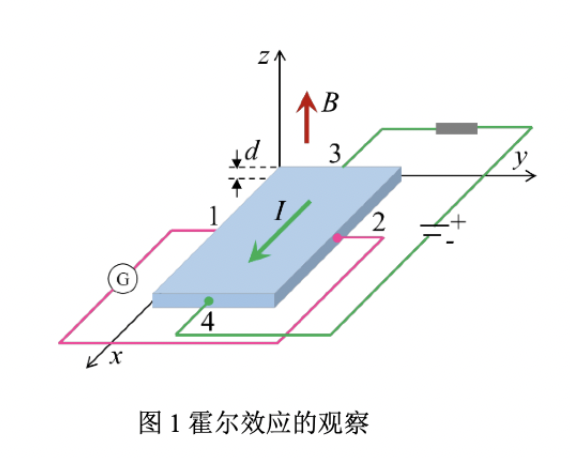
\includegraphics[width=0.8\linewidth]{./image/1.png}
\end{figure}
沿着x轴
正向通以电流I。若在z方向加上磁场B,电流计指针立即偏转,说明1,2两点间产生
了电位差。霍尔发现此电位差与电流强度I和磁感应强度B均成正比,与板厚度成反比,即
\[U_{H}=R_{H}\frac{IB}{d}=K_{H}IB\]
其中$U_{h}$为霍尔电压,$R_{h}$为霍尔系数,$K_{h}=R_{h}/d$为霍尔片的灵敏度.
用洛伦兹力可说明此公式,并可进一步得得到
\[R_{h}=\frac{1}{ne}\]
\[K_{H}=\frac{R_{H}}{d}\]
其中e为载流子电荷,n为载流子浓度.$R_{H}$的单位是$m^{3}/c$.
式(2)和式(3)对大多数金属均成立,但对霍尔系数较高的半导体材料,公式中应引入以一霍尔因子A.在罗磁场的条件下,A=3π/8,故
\[R_{H}=\frac{3\pi}{8}\frac{1}{ne}\]
本次实验为简化计算,A近似为1.
\subsection{霍尔效应的副效应}
实际情况下,会有他一些副效应与霍尔效应混在一起,使霍尔电压的测量产生误差,因此必须尽量消除之.各种效应的特点如下:
\subsubsection{厄廷好森(Etinghausen)效应}
厄廷好森效应所引起的电位差$U_{E}$是指由于载流子以不同的速度在平行于x轴方向上运动,因此在磁场作用下,速度不同于平均速度的载流子在洛伦兹力与霍尔电场力的共同作用下,向y轴方向的两侧偏移,其动能在霍尔片的两侧转化为热能,在两点间产生温差,从而出现温差电动势$U_{E}$.$U_{E}$正比于IB,正负与I,B的方向有关.
\subsubsection{能斯脱(Nernst)效应}
能撕脱效应所引起的电位差$U_{N}$是指由于连接点3,4处接触电阻不同而产生不同的焦耳热,使3,4两点温度不同,从而使载流子在x方向的运动产生热流,它在磁场作用下在1,2两点间产生电位差$U_{N}$.$U_{N}$的符号与磁场B的方向有关.
\subsubsection{里纪-勒杜克(Righi-Ledu)效应}
里纪-勒杜克效应引起的电位差$U_{R}$是指由于上述热流中载流子速度各不相同,在磁场作用下会使1,2两点出现温差电动势$U_{R}$.$U_{R}$方向与B的方向有关.
\subsubsection{不等位效应}
不等位效应引起的电位差$U_0$是指由于制作上的困难,1,2两点不可能恰好处在同一条等位线上,因此只要样品中有电流通过,即使B不存在,1,2两点间也会出现电位差$U_0$.$U_0$的正负只与电流方向有关,其大小在磁场不同时也略不同.
\subsubsection{实际测量}
实际测量时,由于仪表调整的状态,及仪器电压受杂散电磁场和电源地线的影响,电压表会有附加电压$U_{S}$.$U_{S}$与电流,磁场方向无关.


当I,B确定后,霍尔片上的输出电压应为上述几项的代数和
\[U=f(U_{H},U_{E},U_{N},U_{R},U_{0},U_{S})\]
\subsubsection{副效应的消除方法}
通过改变工作电流I的方向和外向磁场B的方向的不同组合测量课消除或减小$U_{N}$,$U_{R}$,$U_0$的影响.$U_{E}$的变化与$U_{H}$变化相同,不能用此法22消除,当$U_{E}$等的值都小于$U_{H}$,实验测量中课略去.消除上述副效应的重点是消除不等位效应$U_{0}$.
\subsection{磁电阻效应原理}
一定条件下,导电材料阻值R岁磁感应强度B的变化规律称为磁阻效应.磁电阻有各种类型,其中正常磁电阻应用很普通,锑化铟传感器是其中一种.正常磁电阻情况下半导体内的载流子受洛伦兹力而偏移,在两端集聚并形成霍尔电场.若霍尔电场作用和某一速度的载流子所受的洛伦兹力刚好抵消,则小于或大于该素的的电子将偏移,沿外加电场方向运动的载流子数目减少,电阻增大,表现出横向磁电阻效应.如图2,若A,B两端短接,则霍尔电场不存在,所有电子将向A断偏转,也表现出磁电阻效应.

设磁阻器件在零磁场时电阻及电阻率分别为$R{O}$,$P(O)$,磁场为B是电阻率分别为$R_{B}$,$\rho(B)$.
以$ \Delta \rho/\rho(O) $表示磁阻,$ \Delta \rho = \rho (B) - \rho(O) $,而$\Delta R /R(O) \propto \Delta \rho /\rho(O)$,
其中
$ \Delta R = R(B)-R(O) $
.磁场较弱时,对正常磁阻器件
$\Delta R /R(O)\propto B^{2}$,而强磁场条件下
$ \Delta R /R(O)$为B的一次函数(如图3).对于实验所用器件,$ B \leq 0.06T$可看做弱磁场条件,$B\geq 0.12T$可看作是强磁场条件.$\Delta R / R(O)$与电源输入端C,D的状态(横流或恒压)及A,B输出端是短路还是开路开关,故实验结果应注明工作条件.
实验中推荐C,D端恒流,A,B端短路的工作条件,因此此时$\Delta R/R(O)$最大.
\section{实~~验~~仪~~器}
\subsection{ZKY-HC霍尔效应测试仪}
包含恒流电源,数字电压表,励磁电流源
\subsection{ZKY-HS霍尔效应测试仪}
包含三组换向开关,电磁铁,霍尔片,磁电阻
\subsection{万用表及导线}
%%%
\section{实~~验~~步~~骤} 
\begin{enumerate}
	\item 测量霍尔片输出电压$U_{H}$与输入电流I的关系曲线,要求电流源2.00\~{}8.00mA,间隔1.00mA,每个测量点
	测量出$$U_{1}(+B,+I_H{}),U_{2}(+B,-I_{H}),U_{3}(_B,-I_{H}),U_{4}(-B,I_{H})$$
	4组数据.可证$U_{H}=\frac{1}{4}(U_{1}-U_{2}+U_{3}-U_{4})$。画出
	$U_{H}$\~{}I关系曲线,计算$K_{H}$,$R_{H}$,n的数值和不确定度,并给出不等位效应$U_{0}$的表示方法.
	\item 标定激励电流$I_{M}$(0\~{}800mA)与磁极间磁场B的关系.
	\item 测定磁极间隙水平方向磁场的的分布曲线B\~{}X,工作电流$ I_{0}=4.00mA,I_{M}=500mA $.
	\item 判定霍尔片载流子的类型是空穴还是电子.实验中记录下$ U_{H},I,B $的方向
	\item 测霍尔片中载流子的迁移率.实验时不加磁场,霍尔片工作电流0\~{}8.00mA改变,同时使用万用表测量C,D端的电压.
	\item 研究锑化铟磁阻器件的磁电阻效应. $C,D$端恒流, $A,B$端短路,$ I_{CD} $=1.50mA.
	\subitem 测磁电阻$ \Delta R/R(0) $随磁场变化规律
	\subitem $ I_{M} $:0\~{}1000mA,间隔50\~{}100mA
	\subitem 前6\~{}8个点为非线性区,间隔50mA
	\subitem 后面为线性区,间隔100mA.
\end{enumerate}
%%%%%%%%%%%%%%%%%%%%%%%%%%%%%%%%%%%%%%%%%%%%%%%%%%%%%%%%%%%%%%%%
\section{注~~意~~事~~项}
\begin{enumerate} 
	\item 避免霍尔元件及二维移动标尺受挤压,碰撞等,实验前检查两者及电磁铁位置并调整.
	\item 实验前应将霍尔元件移至电磁铁气隙中心,并使其平面都与磁场方向垂直,以使$U_{H}$最大.
	\item 在不需要的时候断开励磁电流开关.
\end{enumerate}
%%%%%%%%%%%%%%%%%%%%%%%%%%%%%%%%%%%%%%%%%%%%%%%%%%%%%%%%%%%%%%%%
\section{实~~验~~数~~据}
\begin{figure}[H]
	\centering
	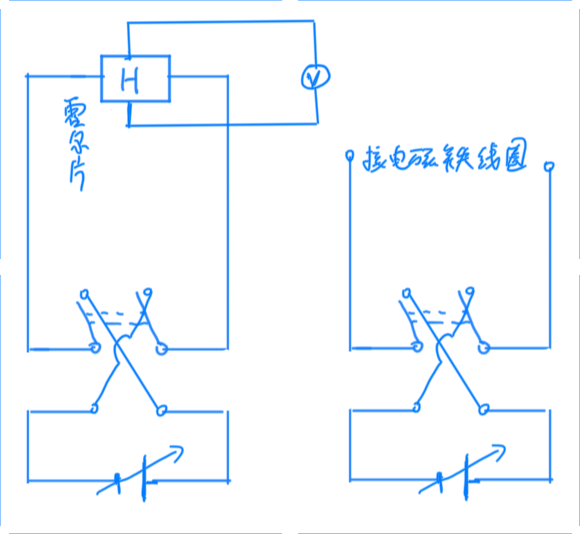
\includegraphics[width=0.8\linewidth]{./image/9.png}
	\caption{实验6.1/6.2/6.3电路图} \label{fig:eg}
\end{figure}
\subsection{$U_{H}$与I关系及$K_{H},R_{H},n$的计算}
实验1中数据整理如下:
\begin{figure}[H]
	\centering
	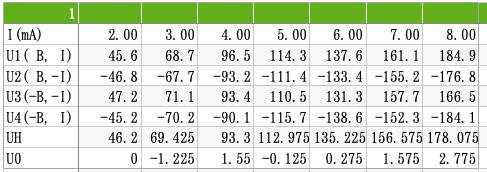
\includegraphics[width=0.8\linewidth]{./image/n1.png}
	\caption{实验1数据} \label{fig:eg}
\end{figure}
由实验室提供的表格查得$I_{M}$=500mA时,$B_{0}$=126.1mT
由实验所测得数据制作的$U_{H}-I$关系曲线如图
\begin{figure}[H]
	\centering
	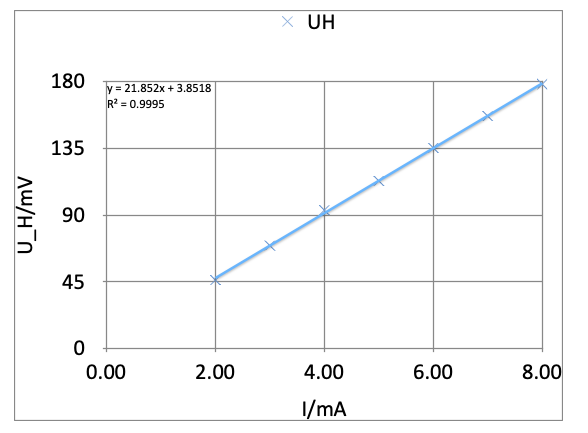
\includegraphics[width=0.8\linewidth]{./image/3.png}
	\caption{$U_{H}$=I} \label{fig:eg}
\end{figure}
可见,$U_{H}$,I成线性关系.

直线斜率k=21.852,相关系数$R^2=0.99995$

由$U_{H}=R_{H}\frac{IB}{d}=K_{H}IB$,故$k=\frac{R_{H}B}{d}=K_{H}$\\所以有
\[R_{H}=\frac{kd}{B}=\frac{23.852\times 3\times 10^{-6}}{123.7x10^{-3}}\approx5.54239x10^{-4} \Omega·m/T\]
\[K_{H}=\frac{k}{B}=187.3256 \Omega/T\]
\[\Delta k =S_{K}=k\sqrt{\frac{\frac{1}{r^{2}-1}}{n-2}}\approx0.04307\Omega\]
\[\Delta R_{H} = \frac{d}{B}\Delta k \approx 1.1x10^{-6} \Omega·m/T\]
\[\Delta K_{H} = \frac{1}{B}\Delta K \approx 0.4\Omega/T\]
故\[R_{H}=(5.551\pm0.011)x10^{-4} \Omega ·m/T\]
\[K_{H}=(187.5\pm 0.4 )\Omega /T\]
又$R_{H}=\frac{1}{ne}$,故\[n=\frac{1}{R_{H}e}=1.1031X10^{22}m^{-3}\]
\[\Delta n =\frac{\Delta R_{H}}{R_{H}^{2}e}\approx2.1x10^{19}m^{-3}\]
故\[n=(1.1031\pm0.0021)X10^{22}m^{-3}\]
不等位效应$U_{0}$的确定:
由实验原理$$U=f(U_{H},U_{E},U_{N},U_{R},U_0,U_{S})$$f表示求和,式中$U_{E}$很小可略去,故
$$U=f(U_{H},U_{E},U_{N},U_{R},U_0,U_{S})=U_{H}+U_{N}+U_{R}+U_{P}+U_{S}$$不妨设+B,+I的条件下参与求和的各电压均取正值
\\由于$U_{H}$正负与I,B方向有关,$U_{N},U_{R}$正负只与B方向有关,$U_0$方向只与I方向有关,$U_{S}$与I,B无关,故
\[U_{1}(+B,+I_{H})=f(U_{H},U_{N},U_{R},U_0,U_{S})\]
\[U_{2}(+B,-I_{H})=f(-U_{H},U_{N},U_{R},-U_0,U_{S})\]
\[U_{3}(-B,-I_{H})=f(U_{H},-U_{N},-U_{R},-U_0,U_{S})\]
\[U_{4}(-B,+I_{H})=f(-U_{H},-U_{N},-U_{R},U_0,U_{S})\]
所以
\[\frac{1}{4}(U_{1}+U_{3}-U_{2}-U_{4}=U_{H}\]
\[\frac{1}{4}[(U_{1}-U_{2})-(U_{3}-U_{4})]=U_0\]
故\[U_0=\frac{1}{4}(U_{1}-U_{2}-U_{3}+U-{4})\]
实验1中结果整理如下:
\[R_{H}=(5.551\pm0.011)\times 10^{-4} \Omega ·m/T,K_{H}=(187.5\pm 0.4 )\Omega /T\]
\[n=(1.1031\pm0.0021)\times 10^{22}m^{-3},U_0=\frac{1}{4}(U_{1}-U_{2}-U_{3}+U-{4})\]
\subsection{标定$I_{M}$与B的关系}
实验2中数据整理如下:
\begin{figure}[H]
	\centering
	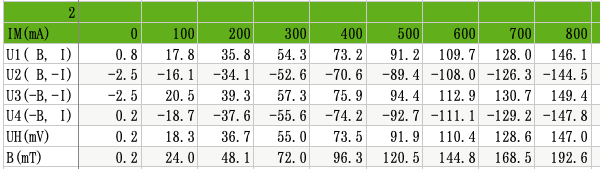
\includegraphics[width=0.8\linewidth]{./image/n2.png}
	\caption{实验2数据} \label{fig:eg}
\end{figure}
有实验数据可得
\[B=\frac{U_{H}}{K_{H}I},I=4.00mA,K_{H}=187.5 \Omega/T\]
由此可作出B-$I_{M}$曲线,
\begin{figure}[H]
	\centering
	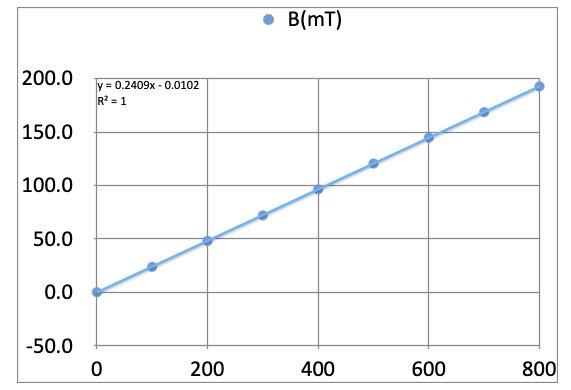
\includegraphics[width=0.8\linewidth]{./image/4.png}
	\caption{B-$I_{M}$} \label{fig:eg}
\end{figure}
由曲线可以看出B与$I_{M}$成线性(基本为正比)关系.
用拟合直线的方程:
\[B=0。2409I_{M}+3.9515\]
$I_{M}$的单位为mA,B单位为mT.
相关系数$R^2=1$

\subsection{磁极间隙水平方向磁场的分布曲线}
实验3中数据整理如下:
\begin{figure}[H]
	\centering
	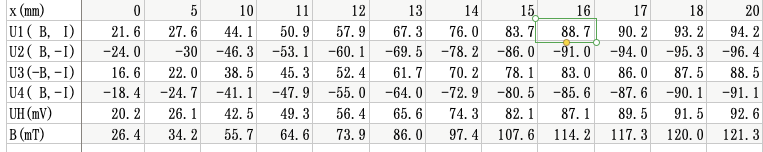
\includegraphics[width=0.8\linewidth]{./image/n4.png}
	\caption{实验5数据1} \label{fig:eg}
\end{figure}
\begin{figure}[H]
	\centering
	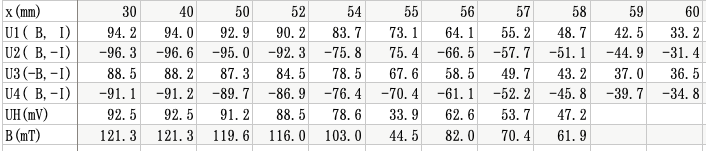
\includegraphics[width=0.8\linewidth]{./image/n5.png}
	\caption{实验5数据2} \label{fig:eg}
\end{figure}
由实验数据整理得:

\[B=\frac{U_{H}}{K_{H}I},I=4.00mA,K_{H}=187.5 \Omega/T\]
	实验时的励磁电流$I_{M}=500mA$
\\可作出实验曲线
\begin{figure}[H]
	\centering
	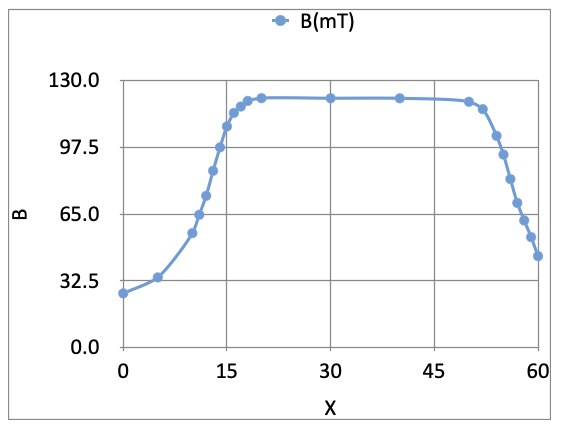
\includegraphics[width=0.8\linewidth]{./image/5.png}
	\caption{B\~{}X} \label{fig:eg}
\end{figure}
曲线有对称性,对称轴大致在气隙中心位置.从曲线中可以看出,随着x的增大,B先是逐渐增大到某个值,在一定范围内保持恒定,然后又逐渐减小.
增加的速度先慢后快,后由快变慢.下降的速度也是这样

从曲线中可以看出,电磁铁气隙中心的磁场为均匀磁场,且磁感应强度最大.
\subsection{判断载流子类型}
\begin{figure}[H]
	\centering
	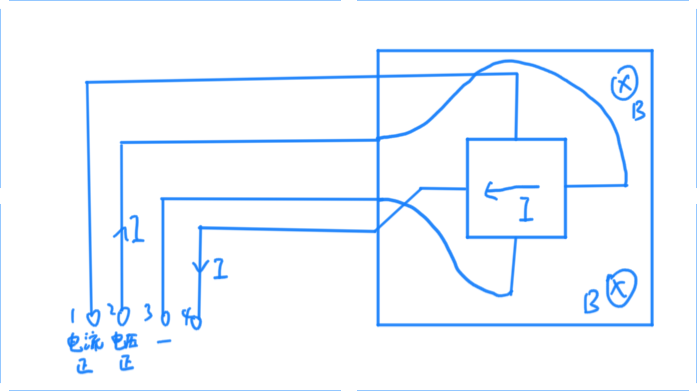
\includegraphics[width=0.8\linewidth]{./image/14.png}
	\caption{载流子类型} \label{fig:eg}
\end{figure}
电流方向如图中标示.由左手定则,不管载流子是电子和空穴,均会发生向下的偏转.有由于3端的电势低,故发生偏转的是电子.也即载流子为电子
\subsection{霍尔片中载流子的迁移率μ}
\begin{figure}[H]
	\centering
	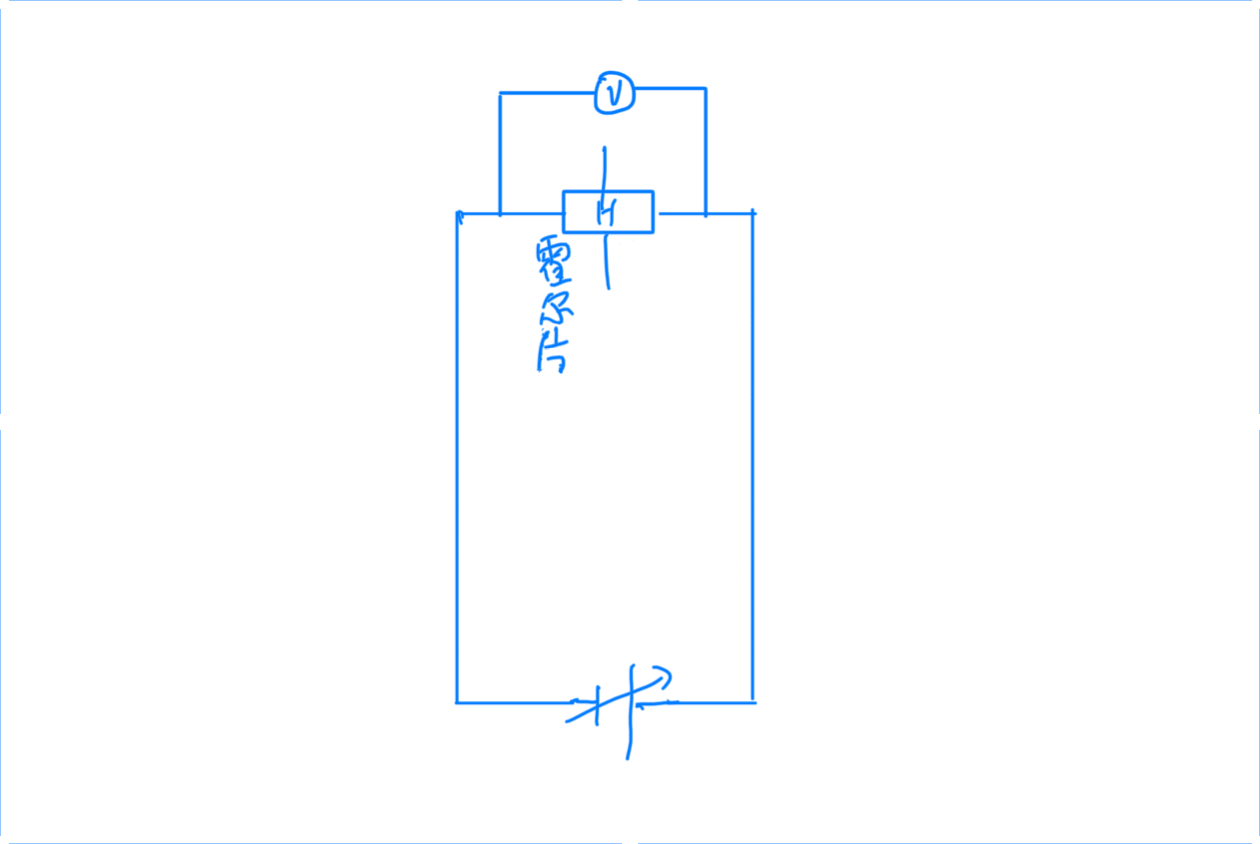
\includegraphics[width=0.8\linewidth]{./image/10.png}
	\caption{实验6.5电路图} \label{fig:eg}
\end{figure}
实验5中数据整理如下:
\begin{figure}[H]
	\centering
	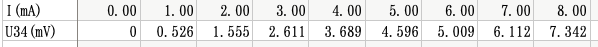
\includegraphics[width=0.8\linewidth]{./image/n6.png}
	\caption{实验5数据} \label{fig:eg}
\end{figure}

\[\mu=\frac{v}{E}=\frac{v}{J/\sigma}=\sigma\frac{v}{nevbd/(bd)}=\frac{\sigma}{ne}=\sigma R_{H}\]
故欲测μ即是要测霍尔片的电导率$\sigma$

又因为电阻R=$ \frac{U_{cd}}{I}=\frac{1}{\sigma}\frac{L}{bd} $

故
\[\sigma = \frac{L}{bd}\frac{I}{U_{cd}},I=\frac{\sigma bd}{l}U_{cd}\]
可见由$I-U_{cd}$的曲线的斜率可求出$\sigma$
\begin{figure}[H]
	\centering
	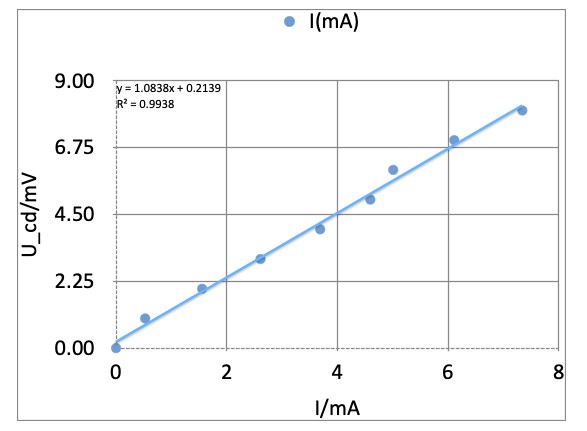
\includegraphics[width=0.8\linewidth]{./image/6.png}
	\caption{载流子迁移率} \label{fig:eg}
\end{figure}
所做图像如图,回归直线方程:$$I=1.0838U_{cd}+0.2139$$
$R^2=0.9938$
故斜率k=1.0838mA/V
\[\Delta k \approx S_{K}=k\sqrt{\frac{1/r^{2}-1}{n-2}}\approx0.010831mA/V\]
\[k=\frac{\sigma bd}{l}\]
\[\sigma=\frac{k l}{b d}\approx1092.6S/m\]
\[\Delta \sigma =\frac{l}{bd}\Delta k\approx11s/m\]
\[\sigma=(1092.6\pm11)S/m\]
\[\mu=\sigma R_{H}=0.618438T^{-1}\]
\[ln\mu=ln\sigma+lnR_{H}\]
\[\frac{\partial ln \mu}{\partial \sigma}=\frac{1}{\sigma},\frac{\partial lu \mu}{\partial R_{H}}=\frac{1}{R_{H}}\]
\[\frac{\Delta \mu}{\mu}=\sqrt{(\frac{\Delta \sigma}{\sigma})^{2}+(\frac{\Delta_{RH}}{R_{H}})^{2}}
=1.0351\times 10^{-2}\]
\[\Delta \mu =\mu \frac{\Delta \mu}{\mu}\approx 6\times 10^{-3}T^{-1}\]
\[\mu=(0.606\pm0.006)T^{-1}\]
\subsection{锑化铟磁阻器件的磁电阻效应}
实验6中数据整理如下:
\begin{figure}[H]
	\centering
	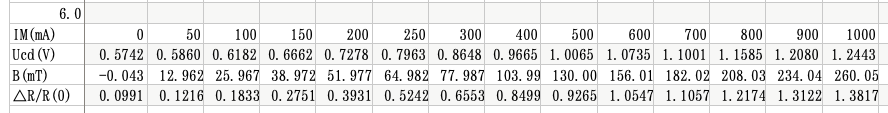
\includegraphics[width=0.8\linewidth]{./image/n3.png}
	\caption{实验6数据1} \label{fig:eg}
\end{figure}

由实验数据由曲线走势进行如下回归分析:\\
取前六点进行二次回归,有
\begin{figure}[H]
	\centering
	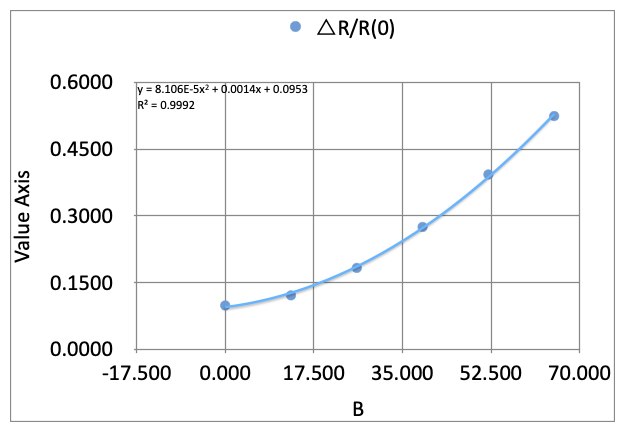
\includegraphics[width=0.8\linewidth]{./image/7.png}
	\caption{$\Delta R/R(O)\~{}B$} \label{fig:eg}
\end{figure}

\[\Delta R/R(O)=0.08016B^{2}+0.0014B+0.0953,R^{2}=0.9992\]
相关程度高

取后六点进行线性回归,有
\begin{figure}[H]
	\centering
	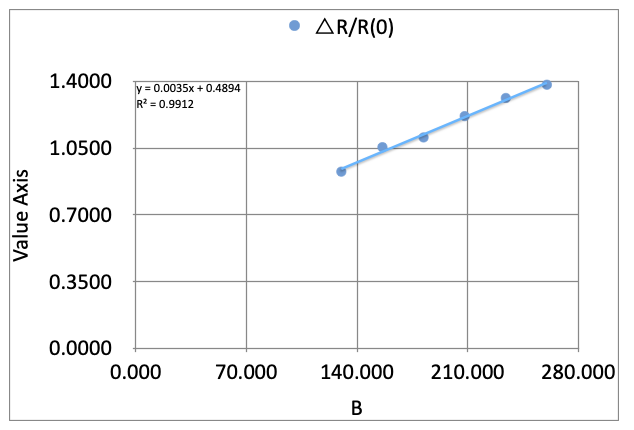
\includegraphics[width=0.8\linewidth]{./image/8.png}
	\caption{$\Delta R/R(O)\~{}B$} \label{fig:eg}
\end{figure}
\[\Delta R/R(0)=0.0035B+0.4894,R^{2}=0.9912\]
相关程度高

于是在\\磁场较弱时,$ \Delta R/R(O) $曲线为抛物线,正比于$B^2$
\\磁场较强时,$ \Delta R/R(O) $存在线性关系,曲线为直线,为B的一次函数关系

实验结果很好的验证了磁电阻效应


%%%%%%%%%%%%%%%%%%%%%%%%%%%%%%%%%%%%%%%%%%%%%%%%%%%%%%%%%%%%%%%%
\section{实~~验~~总~~结}
通过这次实验,我对于霍尔效应有了更加直观,深入的认识.
学会了消除霍尔副效应的方法.
本次实验小实验之间6个联系密切,
实验的数据与电路图的共用让我对这几个实验的体会更加深入。
实验之后对大量的数据处理与作图也让我对于这些工具的使用更加熟练。

同时助教在课程开始时介绍的量子霍尔效应与量子反常霍尔效应也是十分的有趣,让我对于
未来解决摩尔定律的瓶颈问题增加了一些新的思考,拓宽了知识面,十分感谢助教的科普。
%%%%%%%%%%%%%%%%%%%%%%%%%%%%%%%%%%%%%%%%%%%%%%%%%%%%%%%%%%%%%%%%
%  参考文献
%%%%%%%%%%%%%%%%%%%%%%%%%%%%%%%%%%%%%%%%%%%%%%%%%%%%%%%%%%%%%%%%
%  参考文献按GB/T 7714-2015《文后参考文献著录规则》的要求著录. 
%  参考文献在正文中的引用方法:\cite{bib文件条目的第一行}

\renewcommand\refname{\heiti\wuhao\centerline{参考文献}\global\def\refname{参考文献}}
\vskip 12pt

\let\OLDthebibliography\thebibliography
\renewcommand\thebibliography[1]{
  \OLDthebibliography{#1}
  \setlength{\parskip}{0pt}
  \setlength{\itemsep}{0pt plus 0.3ex}
}

{
\renewcommand{\baselinestretch}{0.9}
\liuhao
\bibliographystyle{gbt7714-numerical}
\bibliography{./TempExample}
}


\end{document}
